\documentclass[a4paper]{article}
\usepackage{vntex}
%\usepackage[english,vietnam]{babel}
%\usepackage[utf8]{inputenc}

\usepackage[labelformat=empty]{caption}
\usepackage{vntex}
\usepackage[utf8]{inputenc}
\usepackage{listings}  
\usepackage{tipa}

\lstset{columns=fullflexible,literate=
{ẽ}{{\~e}}1
{ó}{{\'o}}1
{ô}{{\^o}}1
{é}{{\'e}}1
}


\usepackage[english,vietnamese]{babel}
\usepackage[utf8]{inputenc}

%\usepackage[francais]{babel}
\usepackage{a4wide,amssymb,epsfig,latexsym,array,hhline,fancyhdr}
\usepackage[normalem]{ulem}
%\usepackage{soul}
\usepackage{float}
\usepackage[makeroom]{cancel}
\usepackage{amsmath}
\usepackage{amsthm}
\usepackage{multicol,longtable,amscd}
\usepackage{diagbox}%Make diagonal lines in tables
\usepackage{booktabs}
\usepackage{alltt}
\usepackage[framemethod=tikz]{mdframed}% For highlighting paragraph backgrounds
\usepackage{caption,subcaption}

\usepackage{lastpage}
\usepackage[lined,boxed,commentsnumbered]{algorithm2e}
\usepackage{enumerate}
\usepackage{color}
\usepackage{graphicx}							% Standard graphics package
\usepackage{array}
\usepackage{tabularx, caption}
\usepackage{multirow}
\usepackage{multicol}
\usepackage{rotating}
\usepackage{graphics}
\usepackage{geometry}
\usepackage{setspace}
\usepackage{epsfig}
\usepackage{listings}
\usepackage{tikz}
\usetikzlibrary{arrows,snakes,backgrounds}
\usepackage[unicode]{hyperref}
\hypersetup{urlcolor=blue,linkcolor=black,citecolor=black,colorlinks=true} 
%\usepackage{pstcol} 								% PSTricks with the standard color package

\usepackage[normalem]{ulem}

\newtheorem{theorem}{{\bf Định lý}}
\newtheorem{property}{{\bf Tính chất}}
\newtheorem{proposition}{{\bf Mệnh đề}}
\newtheorem{corollary}[proposition]{{\bf Hệ quả}}
\newtheorem{lemma}[proposition]{{\bf Bổ đề}}
\theoremstyle{definition}
\newtheorem{exer}{Bài toán}

\definecolor{codegreen}{rgb}{0,0.6,0}
\definecolor{codegray}{rgb}{0.5,0.5,0.5}
\definecolor{codepurple}{rgb}{0.58,0,0.82}
\definecolor{backcolour}{rgb}{0.95,0.95,0.92}

\lstdefinestyle{mystyle}{
    backgroundcolor=\color{backcolour},   
    commentstyle=\color{codegreen},
    keywordstyle=\color{magenta},
    numberstyle=\tiny\color{codegray},
    stringstyle=\color{codepurple},
    basicstyle=\ttfamily\footnotesize,
    breakatwhitespace=false,         
    breaklines=true,                 
    captionpos=b,                    
    keepspaces=true,                 
    numbers=left,                    
    numbersep=5pt,                  
    showspaces=false,                
    showstringspaces=false,
    showtabs=false,                  
    tabsize=2
}

\lstset{style=mystyle}

\def\thesislayout{	% A4: 210 × 297
	\geometry{
		a4paper,
		total={160mm,240mm},  % fix over page
		left=30mm,
		top=30mm,
	}
}
\thesislayout

%\usepackage{fancyhdr}
\setlength{\headheight}{40pt}
\pagestyle{fancy}
\fancyhead{} % clear all header fields
\fancyhead[L]{
 \begin{tabular}{rl}
    \begin{picture}(25,15)(0,0)
    \put(0,-8){
\includegraphics[width=8mm, height=8mm]{hcmut.png}}
    %\put(0,-8){\epsfig{width=10mm,figure=hcmut.eps}}
   \end{picture}&
	%
\includegraphics[width=8mm, height=8mm]{hcmut.png} & %
	\begin{tabular}{l}
		\textbf{\bf \ttfamily Trường Đại Học Bách Khoa Tp.Hồ Chí Minh}\\
		\textbf{\bf \ttfamily Khoa Khoa Học \& Kỹ Thuật Máy Tính}
	\end{tabular} 	
 \end{tabular}
}
\fancyhead[R]{
	\begin{tabular}{l}
		\tiny \bf \\
		\tiny \bf 
	\end{tabular}  }
\fancyfoot{} % clear all footer fields
\fancyfoot[L]{\scriptsize \ttfamily Báo cáo bài tập lớn môn Xác suất và Thống Kê (MT2013) - Niên khóa 2020-2021}
\fancyfoot[R]{\scriptsize \ttfamily Trang {\thepage}/\pageref{LastPage}}
\renewcommand{\headrulewidth}{0.3pt}
\renewcommand{\footrulewidth}{0.3pt}


%%%
\setcounter{secnumdepth}{4}
\setcounter{tocdepth}{3}
\makeatletter
\newcounter {subsubsubsection}[subsubsection]
\renewcommand\thesubsubsubsection{\thesubsubsection .\@alph\c@subsubsubsection}
\newcommand\subsubsubsection{\@startsection{subsubsubsection}{4}{\z@}%
                                     {-3.25ex\@plus -1ex \@minus -.2ex}%
                                     {1.5ex \@plus .2ex}%
                                     {\normalfont\normalsize\bfseries}}
\newcommand*\l@subsubsubsection{\@dottedtocline{3}{10.0em}{4.1em}}
\newcommand*{\subsubsubsectionmark}[1]{}
\makeatother

\everymath{\color{blue}}%make in-line maths symbols blue to read/check easily

\sloppy
\captionsetup[figure]{labelfont={small,bf},textfont={small,it},belowskip=-1pt,aboveskip=-9pt}
%space remove between caption, figure, and text
\captionsetup[table]{labelfont={small,bf},textfont={small,it},belowskip=-1pt,aboveskip=7pt}
%space remove between caption, table, and text

%\floatplacement{figure}{H}%forced here float placement automatically for figures
%\floatplacement{table}{H}%forced here float placement automatically for table
%the following settings (11 lines) are to remove white space before or after the figures and tables
%\setcounter{topnumber}{2}
%\setcounter{bottomnumber}{2}
%\setcounter{totalnumber}{4}
%\renewcommand{\topfraction}{0.85}
%\renewcommand{\bottomfraction}{0.85}
%\renewcommand{\textfraction}{0.15}
%\renewcommand{\floatpagefraction}{0.8}
%\renewcommand{\textfraction}{0.1}
\setlength{\floatsep}{5pt plus 2pt minus 2pt}
\setlength{\textfloatsep}{5pt plus 2pt minus 2pt}
\setlength{\intextsep}{10pt plus 2pt minus 2pt}

\thesislayout

\begin{document}

\begin{titlepage}
\begin{center}
ĐẠI HỌC QUỐC GIA THÀNH PHỐ HỒ CHÍ MINH \\
TRƯỜNG ĐẠI HỌC BÁCH KHOA \\
KHOA KHOA HỌC \& KỸ THUẬT MÁY TÍNH 
\end{center}

\vspace{1cm}

\begin{figure}[h!]
\begin{center}

\includegraphics[width=3cm]{hcmut.png}
\end{center}
\end{figure}

\vspace{1cm}


\begin{center}
\centering
\begin{tabular}{c}
\multicolumn{1}{l}{\textbf{{\Large XÁC SUẤT VÀ THỐNG KÊ (MT2013)}}}\\
~~\\
\hline
\\
% \multicolumn{1}{l}{\textbf{{\Large Đề bài tập lớn cho Nhóm $n$}}}\\
% \\
% \textbf{{\Huge Thống kê mô tả và}} \\
% \textbf{{\Huge Xác suất rời rạc với R}}\\
    \textbf{\Huge BÀI TẬP LỚN SỐ 2} \\
\\
\hline
\end{tabular}
\end{center}

\vspace{1.5cm}

\begin{table}[h]
\begin{tabular}{rrll}

\hspace{5 cm} & Giảng viên: &  Phan Thị Hường\\
& Lớp: & L16 \\
& Nhóm: & 21\\
& Thành viên:  

& Nguyễn Tấn Đạt & 1911015 \\
&& Nguyễn Trường Hải Đăng & 1911044 \\
&& Lương Thị Quỳnh Hương & 1911314\\
&&Nguyễn Trung Kiên  & 1911441\\
&& Cao Thị Thanh Mai  &     1911565\\
&& Nguyễn Thọ Nam	 & 1911650\\
&& Võ Hồng Phúc & 1911881\\
&& Khổng Mạnh Quyền & 1914881 \\



\end{tabular}
\end{table}
\vspace{1.5cm}
\begin{center}
{\footnotesize Tp. Hồ Chí Minh, tháng 12/2020}
\end{center}
\end{titlepage}


%\thispagestyle{empty}

\newpage
\tableofcontents
\newpage


\section{Phần chung:}
\subsection{Hồi quy tuyến tính bội}\label{code}

\begin{itemize}
	\item Định nghĩa:\\
	Phân tích hồi quy tuyến tính bội là phương pháp phân tích quan hệ giữa biến phụ thuộc Y với nhiều biến độc lập X.\\
	Ta giả sử xây dựng mô hình hồi quy tuyến tính bội cho tổng thể bằng các ma trận sau:\\
		$Y=X\beta+\epsilon$\\
	Với $\beta$ là ma trận các hệ số hồi quy
%	#Nếu các biến số khác trong mô hình không đổi, E(Y) += beta m nếu Xm tăng 1 đơn vị\\
\item Ta đưa ra 4 giả thiết:
\begin{itemize}
    \item Giả thiết 1: Ma trận ngẫu nhiên $\epsilon$ có kì vọng bằng 0.\\
    \item Giả thiết 2: Các thành phần của $\epsilon$ không tương quan\\ 
    $E(\epsilon_i\epsilon_j)=\sigma^2$\\
    \item Giả thiết 3: Các sai số $\epsilon_i$ có phân phối chuẩn $N(0,\sigma^2)\quad \forall i=\overline{1,n}$.\\
	\item 	Giả thiết 4: Các biến độc lập $X_2, X_3,..., X_k$ không có quan hệ tuyến tính.\\
\end{itemize}
\item Ước lượng các hệ số hồi quy:
\begin{itemize}
    \item Phương pháp bình phương bé nhất:
    \begin{itemize}
    \item Lấy  là ước lượng của $\beta$ và $\epsilon$.
        \item Tổng bình phương sai số $SSE=\displaystyle\sum_{i=1}^{n}(y_i-\hat{\y_i})^2$
        \item Tổng các sai số $SE=\displaystyle\sum_{i=1}^{n}(y_i-\hat{\y_i})$
        \item Ta đi tìm đường thằng $\hat{y}=\hat{\beta}X+\hat{\epsilon}$ sao cho SSE là nhỏ nhất, đồng thời SE = 0.
    \end{itemize}
    \item Đo độ biến thiên dữ liệu
    \begin{itemize}
        \item Tổng bình phương toàn phần $SST=\displaystyle\sum_{i=1}^{n}(y_i-\overline{y})^2$
        \item Tổng bình phương hồi quy $SSR=\displaystyle\sum_{i=1}^{n}(\hat{y_i}-\overline{y})^2$
        \item Tổng bình phương sai số $SSE=\displaystyle\sum_{i=1}^{n}(y_i-\hat{y_i})^2$
        \item Hệ số xác định R biểu thị mối liên hệ giữa X và Y: $R^2=\frac{SSR}{SST}$\\
         Tính chất của hệ số xác định $R^2$:
	    \begin{itemize}
	        \item 0$\leq R^2 \leq$1.
	        \item Nếu $R^2$=1 khi đó đường hồi quy giải thích hoàn toàn sự thay đổi của Y bởi vì khi đó:$\displaystyle\sum_{i=1}^{n}\hat{\varepsilon_i}^2=0.$
	        \item Nếu $R^2=0$ khi đó mô hình không giải thích được sự thay đổi của Y.
	        \item Nếu số biến độc lập càng tăng thì hệ số $R^2$ càng lớn, hay nói cách khác $R^2$ là một hàm tăng theo các biến giải thích.\\
	    \end{itemize}
    \end{itemize}
\item Ước lượng phương sai $\sigma^2$ của sai số
Ta có $\frac{SSE}{\sigma^2}~\chi^2(n-2)$
\begin{itemize}
    \item Trung bình bình phương sai số $MSE=\frac{SSE}{n-2}$
    \item Sai số chuẩn của $\sigma^2$ dùng để đo sự biến thiên so với đường thẳng hồi quy: $SE=\sqrt{\frac{SSE}{n-2}}$
     
\end{itemize}
\item Khoảng tin cậy cho hệ số hồi quy
\begin{itemize}
    \item Khoảng ước lượng cho $\beta_i$ là:\\
	$$\hat{\beta_i}-se(\hat{\beta_i})t^{n-k}_{\alpha/2}<\beta_i<\hat{\beta_i}+SE(\hat{\beta_i})t^{n-k}_{\alpha/2};\quad i=\overline{1,k}$$\\
	Với $t^{n-k}_{\alpha/2}$ là phân vị của phân phối Student với (n-k) bậc tự do ứng với mức ý nghĩa $\alpha/2$.\\
\end{itemize}
\item Kiểm định giả thuyết cho các hệ số hồi quy\\
	\\Để so sánh các hệ số hồi quy với các giá trị giả định cho trước, ta có các giả thuyết:
	$$H_0:\beta_i=\beta^*_i \quad i=\overline{1,k}$$
	đi kèm với một trong số các đối thuyết tương ứng $H_1:\beta_i\neq\beta^*_i$ hoặc $H_1:\beta_i>\beta^*_i$ hoặc $H_1:\beta_i<\beta^*_i$.\\
	Với giả thuyết về sai số ngẫu nhiên $\varepsilon$ ta thấy thống kê $t_i=\frac{\hat{\beta_i}-\beta_i^*}{Se(\hat{\beta_i})}$ có phân phối Student với n-k bậc tự do. Dựa vào kết quả đó ta có thể giải quyết một loạt bài toán kiểm định so sánh ước lượng của các hệ số trong mô hình hồi quy tuyến tính bội như sau:\\
	\begin{itemize}
	    \item Bài toán 1:
	    \begin{cases}
	        $H_0:\beta_i=\beta_i^*$\\
	        $H_1:\beta_i\neq\beta_i^*$\\
	    \end{cases}\\
	    Miền bác bỏ: W = $(-\infty;-t^{n-k}_{\alpha/2})\cup(t^{n-k}_{\alpha/2};\infty)$.\\
	    \item Bài toán 2:
	    \begin{cases}
	    
	        $H_0:\beta_i=\beta_i^*$\\
	        $H_1:\beta_i>\beta_i^*$\\
	    \end{cases}\\
	    Miền bác bỏ: W =
	    $(t^{n-k}_{\alpha/2};\infty)$.\\
	    \item Bài toán 3:
	    \begin{cases}
	        $H_0:\beta_i=\beta_i^*$\\
	        $H_1:\beta_i<\beta_i^*$\\
	    \end{cases}\\
	    Miền bác bỏ: W =
	    $(-\infty;-t^{n-k}_{\alpha/2})$.\\
	\end{itemize}
	 Ta có thể tính toán giá trị tiêu chuẩn của thống kê $t_i$ và xác suất ý nghĩa p tương ứng, từ đó có thể giải quyết bài toán theo hai cách sau:\\
	 \begin{itemize}
	     \item Cách 1:\\
	     Tìm phân vị $t^{n-k}_{\alpha/2}$ và miền bác bỏ W rồi so sánh tiêu chuẩn thống kê $t_i$ với W để đưa ra kết luận.\\
	     \item Cách 2:\\
	     So sánh xác suất ý nghĩa p với mức ý nghĩa $\alpha$ đã định trước như sau:\\
	     \begin{itemize}
	         \item Đối với Bài toán 1, nếu $p\neq\alpha$ thì bác bỏ giả thuyết $H_0$, còn nếu $p>\alpha$ thì chấp nhận $H_0$.\\
	         \item Đối với các Bài toán 2 và 3, nếu $p/2\neq\alpha$ thì bác bỏ giả thuyết $H_0$, còn nếu $p/2>\alpha$ thì chấp nhận $H_0$.\\
	     \end{itemize}
	 \end{itemize}
	\end{itemize}
\end{itemize}
\subsection{ANOVA}
\begin{itemize}
    \item Định nghĩa:\\
    \begin{itemize}
        \item Phân tích phương sai (ANOVA) là kỹ thuật thống kê tham số bằng cách tập hợp các mô hình thống kê và các thủ tục ước lượng liên quan của chúng, nhằm phân tích sự khác biệt giữa các nhóm có nghĩa trong một mẫu.\\
        \item Mục tiêu của phân tích phương sai là so sánh trung bình của nhiều nhóm (tổng thể) dựa trên các số trung bình của các mẫu quan sát từ các nhóm này và thông qua sự kiểm định giả thuyết để kết luận về sự bằng nhau của các số trung bình này.\\
        \item Trong nghiên cứu, ANOVA được dùng như một công cụ để xem xét ảnh hưởng của một hay nhiều yếu tố nguyên nhân (định tính) đến một yếu tố kết quả (định lượng).\\
    \end{itemize}
    \item Phân tích phương sai một yếu tố\\
    \begin{itemize}
        \item Là phân tích ảnh hưởng của một yếu tố nguyên nhân đến một yếu tố kết quả (1 biến định tính lên 1 biến định lượng).\\
        \item Giả sư nhân tố A có k mức $X_1,X_2,...,X_k$ với $X_j$ có phân phối chuẩn $N(a,\sigma^2)$ có mẫu điều tra\\
        \\\begin{table}[ht]
            \centering
            \begin{tabular}{c|c|c|c}
 $X_1 & X_2 & ... & X_k$\\
 \hline
 $x_{11} & x_{12} & ... & x_{1k}$\\
 $x_{21} & x_{22} & ... & x_{2k}$\\
 $... & ... & ... & ...$\\
 $x_{n_11} & x_{n_22} & ... & x_{n_kk}$\\
            \end{tabular}
            \label{tab:my_label}
        \end{table}
        Với mức ý nghĩa $\alpha$, hãy kiểm định giả thiết:\\
        \begin{cases}
            $H_0: a_1=a_2=...+a_k$\\
        $H_1:$ "Tồn tại $j_1\neq j_2$ sao cho $a_j_1\neq a_j_2$"
        \end{cases}\\

     \item Nếu $H_0$ đúng thì F=$\frac{MSA}{MSE}$ có phân phối Fisher bậc tự do k-1;n-k.\\
     \item Miền $B_\alpha$: F>$F_{k-1;n-k;1-\alpha}$\\
     Bảng ANOVA
    \end{itemize}
    
    \begin{tabular}{|c|c|c|c|c|}
         \hline
         Nguồn sai số & Tổng bình phương & Bậc tự do & Bình phương trung bình & Giá trị thống kê \\
          & SS & df & MS & F\\
         \hline
         Yếu tố & SSA & k-1 & $MSA=\frac{SSA}{k-1}$ & $F=\frac{MSA}{MSE}$\\
         (Between Group) & & & & \\
         \hline
         Sai số & SSE=SST-SSA & n-k & $MSE=\frac{SSE}{n-k}$ & \\
         (Within Group) & & & & \\
         \hline
         Tổng cộng & SST & n-1 & & \\
         \hline
         \end{tabular}
    \item Phân tích phương sai 2 nhân tố:\\
    Phân tích nhầm đánh giá sự ảnh hưởng của 2 nhân tố A và B trên các giá trị quan sát (biến định lượng) $x_{iJ}$\\
    Giả sử nhân tố
    \begin{itemize}
        \item  A có n mức $a_1,a_2,...,a_n$ (nhân tố hàng)\\
        \item B có m mức $b_1, b_2,..., b_m$ (nhân tố cột)
    \end{itemize}
   \begin{itemize}
       \item Giả thiết $H_0$:
       \begin{itemize}
           \item Tổng thể có phân phối chuẩn
           \item Tổng thể có phương sai bằng nhau.
           \item Mẫu ngẫu nhiên được chọn độc lập
       \end{itemize}
       \item Tiến hành tính toán Tổng giá trị và tổng bình phương của các cột, các hàng và thêm vào cuối bảng.
           \item Đặt T là tổng của tất cả giá trị trong bảng.
           
\item Bảng ANOVA\\
\begin{tabular}{|c|c|c|c|c|}
     \hline
     Nguồn & SS & df & MS & F\\
     \hline
     Yếu tố A & $SSA=\frac{\displaystyle\sum_{i}T^2_{i*}}{m}-\frac{T^2}{m.n}$ & n-1 & $MSA=\frac{SSA}{n-1}$ & $F_A=\frac{MSA}{MSE}$\\
     \hline
     Yếu tố B & $SSB=\frac{\displaystyle\sum_{i}T^2_{*j}}{n}-\frac{T^2}{m.n}$ & m-1 & $MSB=\frac{SSB}{m-1}$ & $F_B=\frac{MSB}{MSE}$\\
     \hline
      & & & & 
     \\Sai số & SSE=SST-SSA-SSB & (n-1)(m-1) & $MSE=\frac{SSE}{(n-1)(m-1)}$ & \\
     \hline
     Tổng & $SST=\displaystyle\sum_{i,j}x^2_{ij}-\frac{T^2}{m.n}$ & nm-1 & & \\
     \hline
\end{tabular}
\item Kết luận
\begin{itemize}
    \item Nếu $F_A>F_{n-1;(n-1)(m-1);1-\alpha}$ thì bác bỏ yếu tố A (hàng).
    \item Nếu $F_B>F_{m-1;(n-1)(m-1);1-\alpha}$ thì bác bỏ yếu tố B (cột).
\end{itemize}
\item Nếu tồn tại nhiều hơn 1 nhân tố quan trắc trông ô, ta ta có mô hình mới gồm:
\begin{itemize}
    \item n nhân tố nhóm A
    \item m nhân tố nhóm B
    \item $\alpha$ quan trắc trong mỗi ô
    \item N là tổng sổ quan trắc của tổng thể.
\end{itemize}
\item Các đặc trưng của phương pháp này có bậc tự do bị thay đổi. Khi ta điều chỉnh được bậc tự do của toàn bộ các giá trị: SST (sự biên thiên toàn phần thành N-1), SSE (sai số thành N-mn), $F_A, F_B$,... ta có thể sử dụng lại phương pháp ANOVA này.
\end{itemize}

\subsection{Bài làm}

    \textbf{Bài tập 1.} Tập tin "\textbf{gia\_nha.csv}" chứa thông tin về giá bán ra thị trường (đơn vị đôla) của 21613 ngôi nhà ở quân King nước Mỹ trong khoảng thời gian từ tháng 5/2014 đến 5/2015. Bên cạnh giá nhà, dữ liệu còn bao gồm các thuộc tính mô tả chất lượng ngôi nhà. Dữ liệu gốc được cung cấp tại: \href{https://www.kaggle.com/harlfoxem/housesalesprediction}{https://www.kaggle.com/harlfoxem/housesalesprediction}.\\ \\
Các biến chính trong bộ dữ liệu:
\begin{itemize}
    
    \item \textbf{price}: Giá nhà được bán ra.
    \item \textbf{sqft\_living15}: Diện tích trung bình của 15 ngôi nhà gần nhất trong khu dân cư.
    \item \textbf{floors}: Số tầng của ngôi nhà được phân loại từ 1 - 3.5.
    \item \textbf{condition}: Điều kiện kiến trúc của ngôi nhà từ 1 $-$ 5, 1: rất tệ và 5: rất tốt.
    \item \textbf{sqft\_above}: Diện tích ngôi nhà.
    \item \textbf{sqft\_living}: Diện tích khuôn viên nhà.
\end{itemize}
\textbf{Câu hỏi:}
\begin{enumerate}
    
    \item \textbf{Đọc dữ liệu (Import data):}
        \begin{itemize}
            \item Phương pháp: dùng lênh \texttt{read.csv()} để đọc tệp tin.
            \item Code:
            \begin{lstlisting}[language=R, caption=Code for question 1]
gianha = read.csv("gia_nha.csv", header=TRUE, sep=",")
            \end{lstlisting}
        \end{itemize}
    
    \item \textbf{Làm sạch dữ liệu (Data cleaning):}
    \begin{enumerate}
        \item  Trích ra một dữ liệu con đặt tên là \textbf{new\_DF} chỉ bao gồm các biến chính mà ta quan tâm như đã trình bày trong phần giới thiệu dữ liệu. Mọi yêu cầu xử lý đều dựa trên tập dữ liệu con \textbf{new\_DF} này.
        
\begin{itemize}
    
    \item Code:
\end{itemize}
        
        \begin{lstlisting}[language=R, caption=Code for question 2a]
#Tao new_DF:
new_DF = data.frame(price = gianha["price"], sqft_living15 =  gianha["sqft_living15"] ,floors = gianha["floors"], condition=gianha["condition"],sqft_above = gianha["sqft_above"], sqft_living = gianha["sqft_living"]) 
        \end{lstlisting}
        
        \item  Kiểm tra các dữ liệu bị khuyết trong tập tin (\textit{Các câu lênh tham khảo:} \texttt{is.na()}, \texttt{which()}, \texttt{apply()}) và đề xuất phương pháp thay thế cho những dữ liệu bị khuyết này.
        
\begin{itemize}
    \item Phương pháp: sử dụng hàm na.omit() để xóa các dòng bị khuyết giá trị.
    \item Code:
\end{itemize}
        
        \begin{lstlisting}[language=R, caption=Code for question 2b]
#Kiem tra cac du lieu bi khuyet va de xuat cac phuong an:
new_DF = na.omit(new_DF) #Xoa hoan toan cac dong bi khuyet gia tri
        \end{lstlisting}
        
    \end{enumerate}
    \item \textbf{Làm rõ dữ liệu (Data visualization):}
    \begin{enumerate}
        \item Chuyển đổi các biến \textbf{price}, \textbf{sqft\_living15}, \textbf{sqft\_above}, \textbf{sqft\_living} lần lượt thành log(\textit{price}), log(\textit{sqft\_living15}), log(\textit{sqft\_above}), và log(\textit{sqft\_living}). Từ đây mọi sự tính toán với các biến trên được hiểu là đã qua đổi biến dạng log.
        
        \begin{itemize}
            \item Code:
        \end{itemize}
        
    \begin{lstlisting}[language=R, caption=Code for question 3a]
#Chuyen doi sang log:
new_DF["price"]=log(new_DF["price"])
new_DF["sqft_living15"]=log(new_DF["sqft_living15"])
new_DF["sqft_living"]=log(new_DF["sqft_living"])
new_DF["sqft_above"]=log(new_DF["sqft_above"])
    \end{lstlisting}   
        
        
        \item Đối với các biến liên tục, tính các giá trị thống kê mô tả bao gồm: trung bình, trung vị, độ lệch chuẩn, giá trị lớn nhất và giá trị nhỏ nhất. Xuất kết quả dưới dạng bảng. (Hàm gợi ý:\texttt{ mean(), median(), sd(), min(), max() , apply(), as.data.frame(), rownames()}).
        
        \begin{itemize}
            \item Code:
            \begin{lstlisting}[language=R, caption=Code for question 3b]
#Tinh cac gia tri thong ke va xuat ra dang bang:
Values = data.frame(
    INFOR = c("price","sqft_living15","sqft_above","sqft_living"),
    MEAN = c(mean(new_DF$price),mean(new_DF$sqft_living15),mean(new_DF$sqft_above),mean(new_DF$sqft_living)), 
    MEDIAN = c(median(new_DF$price),median(new_DF$sqft_living15),median(new_DF$sqft_above),median(new_DF$sqft_living)),
    SD = c(sd(new_DF$price),sd(new_DF$sqft_living15),sd(new_DF$sqft_above),sd(new_DF$sqft_living)),
    MIN = c(min(new_DF$price),min(new_DF$sqft_living15),min(new_DF$sqft_above),min(new_DF$sqft_living)),
    MAX = c(max(new_DF$price),max(new_DF$sqft_living15),max(new_DF$sqft_above),max(new_DF$sqft_living))
    )
Values
            \end{lstlisting} 
            \item Kết quả được in ra màn hình:
            \begin{figure}[H]
            \centering
            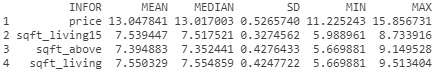
\includegraphics[scale=0.7]{3b.png}
            \label{fig:my_label}
        \end{figure}    
            \begin{center}
                \textbf{Hình 1:} \textit{Tính toán các giá trị thống kê mô tả.}
            \end{center}
        \end{itemize}
        Dựa trên các thông số trên bảng, ta đưa ra một số nhận xét:
        \begin{itemize}
            \item Giá trị mean và median không chênh lệch lớn.
            \item Các thông số biến động không lớn so với giá trị trung bình của chúng.
            \item Giá trị Min max tương đối đối xứng qua hình dạng phân phối chuẩn
            \item Đây là một mẫu có các thông số ổn định, không chênh lệch lớn. Điều này chứng tỏ không có biến động hoặc điều gì đó bất thường đối với các nhân tố được xem xét.
        \end{itemize}
        \item Đối với các biến phân loại, lập một bảng thống kê số lượng cho từng chủng loại (sử dụng hàm \texttt{table()}).
        
        \begin{itemize}
            \item Code:
            \begin{lstlisting}[language=R, caption=Code for question 3c]
#Thong ke so luong cho tung chung loai            
table(new_DF$floors)
table(new_DF$condition)            \end{lstlisting}
            \item Kết quả được in ra màn hình:
            \begin{figure}[H]
            \centering
            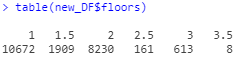
\includegraphics[scale=0.7]{3cfloors.png}
            \label{fig:my_label}
        \end{figure}  
        \begin{center}
            \textbf{Hình 2: }\textit{Bảng thống kê số lượng nhà theo số tầng của ngôi nhà}
        \end{center}
        
        \begin{figure}[H]
            \centering
            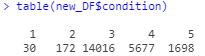
\includegraphics[scale=0.7]{3ccondition.png}
            \label{fig:my_label}
        \end{figure}  
        
        \begin{center}
            \textbf{Hình 3: }\textit{Bảng thống kê số lượng nha theo điều kiện kiến trúc của ngôi nhà}
            \end{center}
            
        \end{itemize}
\item Nhận xét: 
\begin{itemize}
    \item Các căn nhà chủ yếu tập trung ở số tầng thấp (từ 1 tới 2) và ở mức điều kiện kiến trúc trung bình (mức 3-4).
    \item Xu hướng của người mua nhà có thể là các ngôi nhà cho người có điều kiện trung bình và gia đình nhỏ (Ví dụ như công nhân, người già...)
\end{itemize}
        
        \item Dùng hàm \texttt{hist()} để vẽ đồ thị phân phối của biến \textbf{price}.
        
        \begin{itemize}
            \item Code:
            
            \begin{lstlisting}[language=R, caption=Code for question 3d]
#Ve do thi phan phoi cua bien price            
hist(new_DF$price,main="Do thi phan phoi cua bien price",xlab="Price")
            \end{lstlisting}
            
            \item Kết quả được in ra màn hình:
            
            \begin{figure}[H]
            \centering
            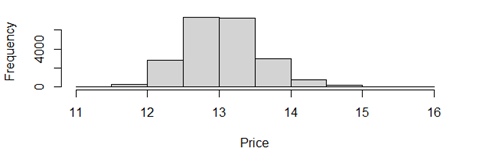
\includegraphics[scale=0.7]{3d.png}
            \label{fig:my_label}
        \end{figure} 
        
        \begin{center}
            \textbf{Hình 4: }\textit{Đồ thị phân phối của biến price}
        \end{center}
            
        \end{itemize}
        Nhận xét:\\
        \begin{itemize}
            \item Đồ thị phân bố của Price có hình dạng đối xứng với trục đối xứng là giá trị 13 đặt tại trung vị của biến.
            \item Thông qua hình dạng phân phối này, ta nhận ra xu hướng chọn mua nhà của người mua thường dao động quanh giá trị trung vị và tần số này giảm dần khi càng ra xa giá trị trung vị này.
        \end{itemize}
        \item Dùng hàm \texttt{boxplot()} vẽ phân phối của biến \textbf{price} cho từng nhóm phân loại của biến \textbf{floors} và biến \textbf{condition}
        
        \begin{itemize}
            \item Code:
            \begin{lstlisting}[language=R, caption=Code for question 3e]
#Phan phoi cua bien price cho tung nhom phan loai cua bien floors
boxplot(new_DF$price ~ new_DF$floors,
        main="different boxplots for each floors",
        xlab="floors",
        ylab="price",
        col="orange",
        border="brown")
#Phan phoi cua bien price cho tung nhom phan loai cua bien condition
boxplot(new_DF$price~new_DF$condition,
        main="different boxplots for each condition",
        xlab="condition",
        ylab="price",
        col="orange",
        border="brown")
            \end{lstlisting} 
            
            \item Kết quả được in ra màn hình:
            
            \begin{figure}[H]
            \centering
            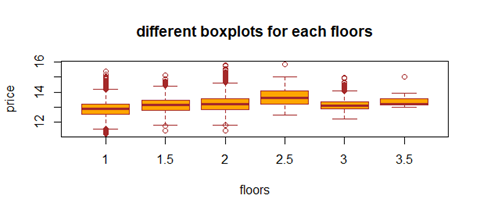
\includegraphics[scale=0.7]{3efloors.png}
            \label{fig:my_label}
            \end{figure}
        
            \begin{center}
            \textbf{Hình 5: }\textit{Phân phối biến price theo từng nhóm phân loại của biến floors}
            \end{center}
        
            \begin{figure}[H]
            \centering
            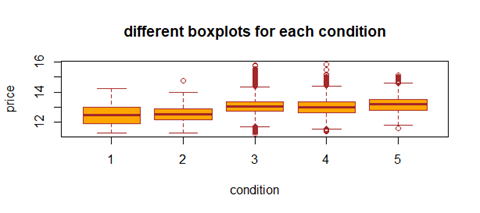
\includegraphics[scale=0.7]{3econdition.png}
            \label{fig:my_label}
            \end{figure}
            
            \begin{center}
            \textbf{Hình 5: }\textit{Phân phối biến price theo từng nhóm phân loại của biến condition}
            \end{center}
            
        \end{itemize}
        Nhận xét:
        \begin{itemize}
            \item Giá nhà tuy có trung vị khá ổn định trong mỗi mô hình, song lại tồn tại rất nhiều Outliers gây ra sự ngẫu nhiên. Vì vậy, Price và floors hoặc condition đều không có mối tương quan hồi quy đơn.
           
            \item Tại các điểm như floors = 1 hoặc condition = 3, các điểm ngoại lai xuất hiện với tần số lớn hơn thể hiện sự tương quan của biến giá nhà với các biến còn lại chưa được xét đến trong mỗi đồ thị đơn.
        \end{itemize}
    
        \item Dùng lệnh \texttt{pairs()} vẽ các phân phối của biến \textbf{price} lần lượt theo các biến \textbf{sqft\_living15}, \textbf{sqft\_above} và \textbf{sqft\_living}
        
        \begin{itemize}
            \item Code:
            
            \begin{lstlisting}[language=R, caption=Code for question 3f]
#Phan phoi cua bien price lan luot theo cac bien sqft_living15, sqft_above va sqft_living
pairs(new_DF$price~new_DF$sqft_living+new_DF$sqft_above+new_DF$sqft_living15, col="red", pch = 18, labels = c("price", "sqft_living","sqft_above","sqft_living15")) 
            \end{lstlisting} 
            
            \item Kết quả được in ra màn hình:
            \begin{figure}[H]
                \centering
                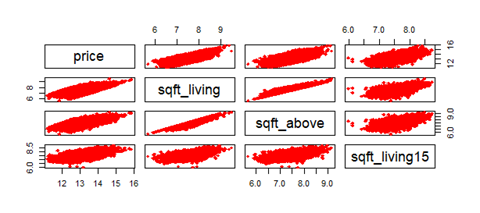
\includegraphics[scale = 0.8]{3f.png}
                \label{fig:my_label}
            \end{figure}
            
            \begin{center}
                \textbf{Hình 5: }\textit{Phân phối của biến \textbf{price} lần lượt theo các biến \textbf{sqft\_living15}, \textbf{sqft\_above} và \textbf{sqft\_living}.}
            \end{center}
            
        \end{itemize}
    Nhận xét:\\
    \begin{itemize}
        \item Giá trị của biến price phân bố ngẫu nhiên trên các đồ thị hàm pairs chứng tỏ biến price không được biểu thị trực tiếp bằng một hàm hồi quy tuyến tính một biến.
        \item Nhờ sự tính ngẫu nhiên cao của các đơn mô hình, ta sẽ xây dựng mô hình hồi quy tuyến tính bội đối với biên price ở mục 4.
    \end{itemize}
            
    \end{enumerate}
    \item \textbf{Xây dựng các mô hình hồi quy tuyến tính (Fitting linear regression models):} \\
    \noindent Chúng ta muốn khám phá rằng có những nhân tố nào và tác động như thế nào đến giá nhà ở quận King.
    \begin{enumerate}
        \item Xét mô hình hồi quy tuyến tính bao gồm biến \textbf{price} là một biến phụ thuộc, và tất cả các biến còn lại đều là biến độc lập. Dùng lệnh \texttt{lm()} để thực thi mô hình hồi quy tuyến tính bội.
        
        \begin{itemize}
            \item Code:
            
            \begin{lstlisting}[language=R, caption=Code for question 4a]
#Chu thich        
hoiqui1=lm(price ~. , data=new_DF )
summary(hoiqui1)                
            \end{lstlisting}
            
            \item Kết quả được in ra màn hình:
            
            \begin{figure}[H]
            \centering
            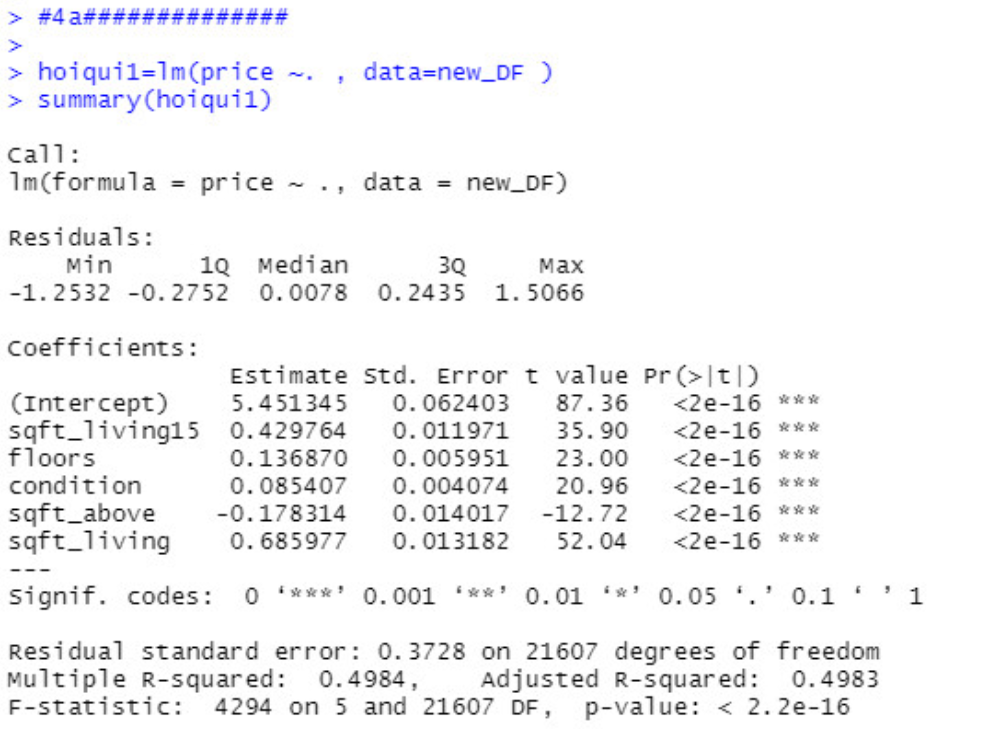
\includegraphics[scale=0.3]{4a.png}
            \label{fig:my_label}
            \end{figure}
        
            \begin{center}
            \textbf{Hình 6: }\textit{Caption}
            \end{center}
            
        \end{itemize}
       
        \item Dựa vào kết quả của mô hình hồi quy tuyến tính trên, những biến nào bạn sẽ loại khỏi mô hình tương ứng với mức tin cậy 5\%.
        
        Ta có $t_0.05$ = 2.365\\
        So sánh với tất cả các giá trị t của từng biến trong bảng trên, ta loại đi giá trị t = -12.72 của biến sqrt\_above.\\
        Nhận xét: Do biến sqrt\_above có độ tin cậy thấp, việc loại bỏ biến này có thể giúp mô hình đơn giản hơn.
        Ngoài ra, vì tất cả các biến đều có độ quan trọng cao nên ta sẽ giữ lại các biến có t value dương.
        \item  Xét 2 mô hình tuyến tính cùng bao gồm biến \textbf{price} là biến phụ thuộc nhưng:
        
        
        \begin{itemize}
            \item Mô hình M1 chứa tất cả các biến còn lại là biến độc lập.
            \item Mô hình M2 là loại bỏ biến \textbf{condition} từ mô hình M1.
        \end{itemize}   
        Dùng lệnhh \texttt{anova()} để đề xuất mô hình hồi quy hợp lý hơn.
        
        \begin{itemize}
            \item Code:
            
            \begin{lstlisting}[language=R, caption=Code for question 4c]
#Mo hinh M2 da loai bo bien condition tu mo hinh M1       
hoiqui2=lm(price ~ sqft_living15 + sqft_above 
          + sqft_living + floors, data=new_DF )
summary(hoiqui2) 

 
CONDITION=as.factor(new_DF$condition)
PRICE=new_DF$price
anova1=data.frame(CONDITION,PRICE)
price.anova1=anova(lm(PRICE~CONDITION,data=anova1 ))
#p-value=3.168169e-64 < alpha=0,05 -> bac bo H0 -> mo hinh 1 hop ly hon
            \end{lstlisting}
            
            \item Kết quả được in ra màn hình:
            
            \begin{figure}[H]
                \centering
                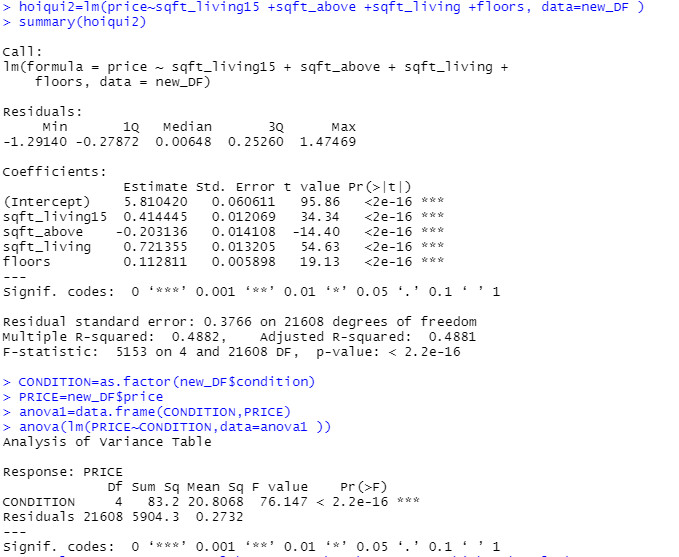
\includegraphics[scale=0.7]{4f.jpg}
                \label{fig:my_label}
            \end{figure}
        
            \begin{center}
                \textbf{Hình 7: }\textit{Loại bỏ đi biến Condition}
            \end{center}
            
        \end{itemize}
        
        
        \item  Chọn mô hình hợp lý hơn từ câu (c) hãy suy luận sự tác động của các biến lên giá nhà.
        
        Từ anova, thông qua giá trị P-value và Coefficient cho thấy mọi giá trị condition đều đóng vai trò quan trọng. Vì vậy, ta khồng thể loại bỏ mô hình biến trên và buộc phải chọn lựa mô hình 1.
        
        \item Từ mô hình hồi quy mà bạn chọn ở câu (c) dùng lệnh \texttt{plot()} để vẽ đồ thị biểu thị sai số hồi quy (residuals) và giá trị dự báo (fitted values). Nêu ý nghĩa và nhận xét đồ thị.
        
        \begin{itemize}
            \item Code:
            \begin{lstlisting}[language=R, caption=Code for question 4e]
#Ve do thi sai so hoi quy va gia tri du bao
resid(hoiqui1)
fitted(hoiqui1) 
op <- par(mfrow=c(2,2)) #yeu cau R danh ra 4 cua so
plot(hoiqui1) #ve cac do thi trong reg
        \end{lstlisting}
        
            \item Kết quả được in ra màn hình:
                \begin{figure}[H]
                \centering
                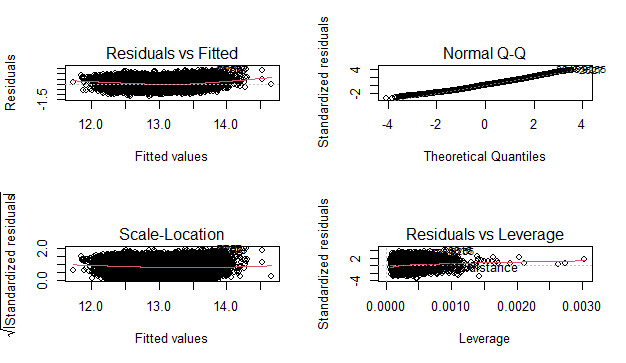
\includegraphics[scale=0.7]{4e.jpg}
                \label{fig:my_label}
                \end{figure}

            \begin{center}
                \textbf{Hình 8: }\textit{Đồ thị biểu thị sai số hồi quy (residuals) và giá trị dự báo (fitted values).}
            \end{center}
        
            \item Nêu ý nghĩa và nhận xét đồ thị:
            \begin{itemize}
                \item Sai số hồi quy ước lượng các điểm mà ta chưa quan sát được trong mẫu.
                \item Sai số chuẩn hoá thể hiện độ lệch của các điểm nằm trong mẫu và điểm ước lượng.
                \item Ta sử dụng các đồ thị này để xem xét số các điểm outliers không tuân theo mô hình hồi quy này.
                \item  Sai số và sai số chuẩn hoá (Standardized Residual) phân bố ngẫu nhiên trên các đổ thị tương quan với giá trị dự báo.
                \begin{itemize}
                    \item Giá trị của sai số là các điểm ngẫu nhiên và tương đối đối xứng quanh 0. Đường giá trị này tương ứng với mô hình hồi quy.
                    \item Các điểm ngoại lệ có tần số rất thấp nên có thể bỏ qua.
                    \item Hình dạng của đồ thị QQ chứng minh cho ta rằng giá trị của phần dư chuẩn hoá là một phân phối chuẩn.
                \end{itemize}
            \end{itemize}
        \end{itemize}

    \end{enumerate}
    
    \item \textbf{Dự báo (Predictions):} \\
    Từ mô hình bạn chọn trong câu (c), hãy dùng lệnh \texttt{predict()} để dự báo giá nhà tại 2 thuộc tính như sau:
    \begin{itemize}
        \item[] x1: sqft\_living15 = mean(sqft\_living15), sqft\_above = mean(sqft\_above), sqft\_living = mean(sqft\_living), floor = 2, condition = 3.
        \item[] x2: sqft\_living15 = max(sqft\_living15), sqft\_above = max(sqft\_above), sqft\_living = max(sqft\_living), floor = 2, condition = 3.
    \end{itemize}
    So sánh khoảng tin cậy cho 2 giá trị dự báo này.
    
    \begin{itemize}
            \item Code:
        \end{itemize}
    
        \begin{lstlisting}[language=R, caption=Code for question 5]
#Chu thich        
predict(hoiqui1, 
        data.frame(sqft_living15 = mean(new_DF$sqft_living15), 
                   sqft_above = mean(new_DF$sqft_above), 
                   sqft_living= mean(new_DF$sqft_living), 
                   floors = c(2), condition = 3))
predict(hoiqui1, 
        data.frame(sqft_living15 = max(new_DF$sqft_living15), 
                   sqft_above = max(new_DF$sqft_above), 
                   sqft_living= max(new_DF$sqft_living), 
                   floors = c(2), condition = 3))
        \end{lstlisting} 
        
        \begin{figure}[H]
            \centering
            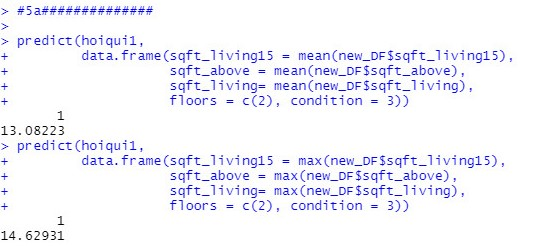
\includegraphics[scale=0.8]{5a.jpg}
            \label{fig:my_label}
        \end{figure}
        
        \begin{center}
            \textbf{Hình 9: }\textit{Giá nhà với hai thuộc tính đã cho.}
        \end{center}
                    
    \end{enumerate}



\section{Phần riêng}\label{objective}
\subsection{Mô tả dữ liệu}
Số liệu mua sắm trực tuyến của sinh viên trên Shopee. Số liệu thu được gồm có các nội dung sau đây:
\begin{itemize}
    \item Thông tin về khách hàng làm khảo sát:
    \begin{itemize}
        \item Sinh viên năm mấy?
        \item Giới tính
        \item Chi tiêu trong tháng?
        \item Số lượng khách hàng chọn 5 trang mua sắm trực tuyến phổ biến hiện nay (Shopee, Tiki, Lazada, Adayroi, Sendo)
        \item Số lần mua sắm hàng hóa trên các nền tảng trực tuyến trong 1 tháng
        \item Hình thức thanh toán
        \item Lý do chọn mua sắm trực tuyến
        \begin{itemize}
            \item Giá thành hợp lý
            \item Tiết kiệm thời gian
            \item Sản phẩm đa dạng và phong phú
            \item Các chương trình khuyến mãi
        \end{itemize}
        \item Có tìm kiếm thông tin trước khi mua sắm trên Shopee hay không? Tìm kiếm qua phương tiện nào?
         \begin{itemize}
            \item Công cụ tìm kiếm online (Google, Bing,..)
            \item Mạng xã hội
         \end{itemize}
        \item Các yếu tố quan tâm khi mua sắm hàng hóa trên Shopee
        \begin{itemize}
            \item Chất lượng sản phẩm đảm bảo
            \item Cách thức thanh toán, giao nhận hàng
            \item Thương hiệu sản phẩm
            \item Giá thành sản phẩm
        \end{itemize}
        \item Trong tương lai có dự định sẽ tiếp tục sử dụng Shopee không?
    \end{itemize}
    \item Đánh giá các dịch vụ của Shopee:
    \begin{itemize}
        \item Chất lượng sản phẩm có đảm bảo không?
        \item Các sản phẩm trên Shopee có đáp ứng được nhu cầu mua sắm của khách hàng không?
        \item Thời gian vận chuyển có làm khách hàng hài lòng?
        \item Khách hàng có yên tâm về chính sách đổi/trả hàng của Shopee?
        \item Giao diện Shopee có giúp khách hàng dễ tiếp cận và mua sắm không?
    \end{itemize}
\end{itemize}
\newpage
\subsection{Làm rõ dữ liệu:}
    \begin{itemize}
    \item Nhập dữ liệu
    \begin{enumerate}
\item Nạp file và đổi tên biến để thuận tiện thao tác.
\begin{lstlisting}[language=R, caption=Nhập dữ liệu]
set_col_name <- function(df){
  colnames(df)[1] <- "Time"
  colnames(df)[7] <- "Freq"
  colnames(df)[8] <- "Proper_Price"
  colnames(df)[9] <- "Time_saving"
  colnames(df)[10] <- "Da_dang"
  colnames(df)[11] <- "Khuyen_Mai"
  colnames(df)[12] <- "Thiet_bi_di_dong"
  colnames(df)[13] <- "Web"
  colnames(df)[14] <- "Social_network"
  colnames(df)[15] <- "Thiet_bi_dien_tu"
  colnames(df)[16] <- "Quan_tam_chat_luong"
  colnames(df)[17] <- "Quan_tam_thanh_toan"
  colnames(df)[18] <- "Quan_tam_thuong_hieu"
  colnames(df)[19] <- "Quan_tam_gia_ca"
  colnames(df)[20] <- "Payment"
  colnames(df)[21] <- "Su_dung_tiep"
  colnames(df)[22] <- "Giao_dien"
  colnames(df)[23] <- "Nhu_cau"
  colnames(df)[24] <- "Chat_luong"
  colnames(df)[25] <- "Dich_vu"
  colnames(df)[26] <- "De_dang"
  colnames(df)[27] <- "Anh_huong_gia_ca"
  colnames(df)[28] <- "Nguon_goc"
  colnames(df)[29] <- "Vuot_troi_hon"
  colnames(df)[30] <- "courier_time"
  colnames(df)[31] <- "Uy_tin"
  colnames(df)[32] <- "Marketing"
  colnames(df)[33] <- "Sale"
  colnames(df)[34] <- "Danh_gia_dich_vu"
  colnames(df)[35] <- "Sinh_vien_nam"
  colnames(df)[36] <- "Gender"
  colnames(df)[37] <- "Chi_tieu"
  return(df)
}
Excel <- read_excel("Input.xlsx")
Excel = set_col_name((Excel))
\end{lstlisting}
\newpage 
    \begin{figure}[H]
        \centering
        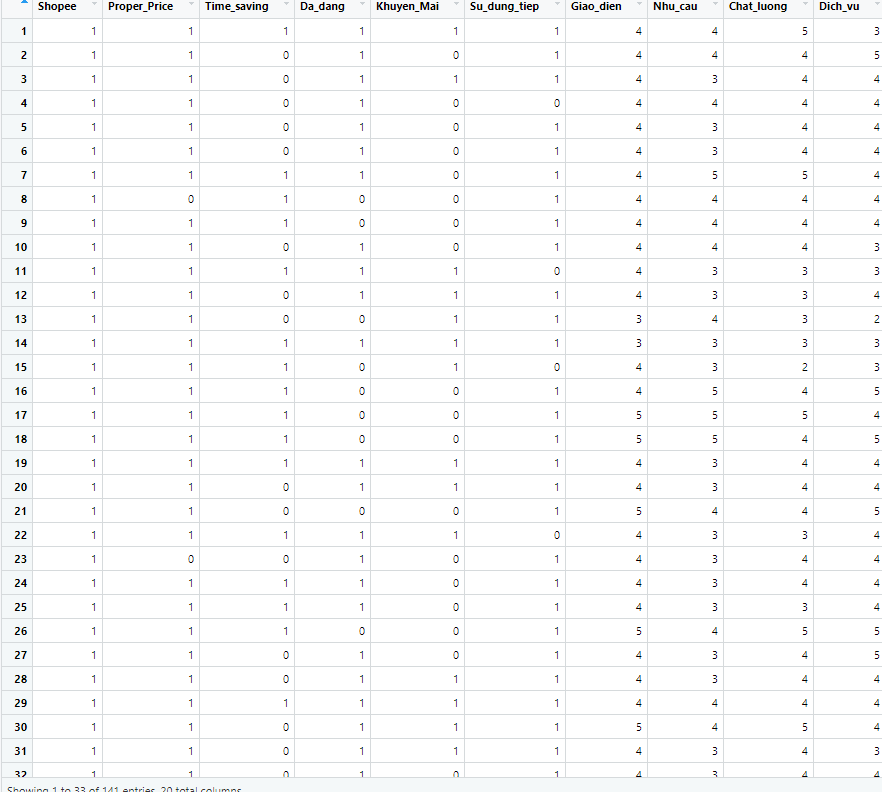
\includegraphics[scale=0.55]{rieng_1.png}
        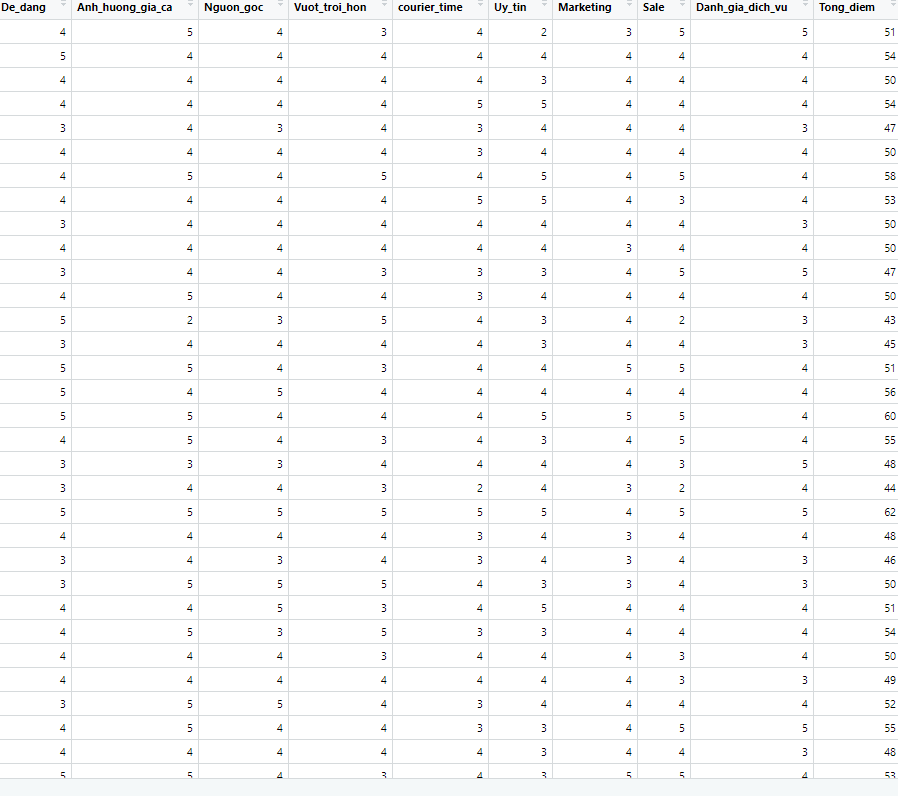
\includegraphics[scale=0.55]{rieng_2.png}
        \label{fig:my_label}
    \end{figure}
    
    \begin{center}
        \textbf{Hình 1: }\textit{Bảng data chúng ta sẽ làm việc}
    \end{center}
\item Thao tác lấy các giá trị quan tâm liên quan đến Shopee. \\
Tại đây, các thông số cần thiết sẽ được ghép với nhau tạo thành dataframe mới có tên là data.\\
\textit{Cú pháp lệnh được sử dụng:}\\
\texttt {> X <- cbind ( arg1, arg2, arg3,... )}
\begin{lstlisting}[language=R, caption=Nhập dữ liệu (tiếp theo)]
data <- cbind(Excel[][2], Excel[][8:11], Excel[][21:34])
\end{lstlisting}
\item Loại bỏ hết các giá trị NA.\\
Bằng cách rà soát từng cột của bảng và cập nhật dữ liệu của từng cột trong bảng, ta thu được data mới không chứa các dữ liệu mang giá trị NA.\\
\textit{Cú pháp 2 lệnh được sử dụng:}
\begin{itemize}
    \item \texttt{ > for ( variable in expression1 ) expression2}
    \item \texttt{ > subset ( data, cond )}
\end{itemize}
\begin{lstlisting}[language=R, caption=Nhập dữ liệu (tiếp theo)]
for(i in 1:19) {
  data <- subset(data, !is.na(data[][i]))
}
\end{lstlisting}
\item Đổi lại thông số trong cột sử dụng tiếp thành số để thao tác phân tích: 
\begin{lstlisting}[language=R, caption=Nhập dữ liệu (tiếp theo)]
data$Su_dung_tiep[data$Shopee == 0] = 0
data$Su_dung_tiep[data$Su_dung_tiep == "Có"] = 1
data$Su_dung_tiep[data$Su_dung_tiep == "Không"] = -1
data$Su_dung_tiep[data$Su_dung_tiep == "Sẽ xem xét"] = 0
data$Su_dung_tiep = as.numeric(data$Su_dung_tiep)
\end{lstlisting}
\item Tính toán giá trị Tổng điểm nhằm mục đích mô hình dữ liệu
\begin{lstlisting}[language=R, caption=Nhập dữ liệu (tiếp theo)]
temp <- data[][7]
colnames(temp)[1] = "Tong_diem"
for(i in 8:19) {
  temp <- temp[][1] + data[][i]
}
data <- cbind(data, temp)
View(data)
\end{lstlisting}
\end{enumerate}
\item Làm rõ dữ liệu
\begin{enumerate}
\item Đối với các biến định lượng\\
\begin{itemize}
    \item Tìm min, max, sd, median, average:\\
    Ta sử dụng các hàm min, max, median... có sẵn  và chứa giá trị vào các tên biến tương đương\\
\begin{lstlisting}[language=R, caption=Làm rõ dữ liệu]
#VOI CAC BIEN DANH GIA BANG DIEM
Average = apply(data[7:20], 2, mean)
Median= apply(data[7:20], 2, median)
SD = apply(data[7:20], 2, sd)
Max = apply(data[7:20], 2, max)
Min = apply(data[7:20], 2, min)
\end{lstlisting}
\item Đưa các thông số này về một bảng\\
\begin{lstlisting}[language=R, caption=Làm rõ dữ liệu (tiếp theo)]
statistical_table1 <- cbind(Average, Median)
statistical_table1 <- cbind(statistical_table1, SD)
statistical_table1 <- cbind(statistical_table1, Max)
statistical_table1 <- cbind(statistical_table1, Min)
View(statistical_table1)
\end{lstlisting}
        \begin{figure}[H]
            \centering
            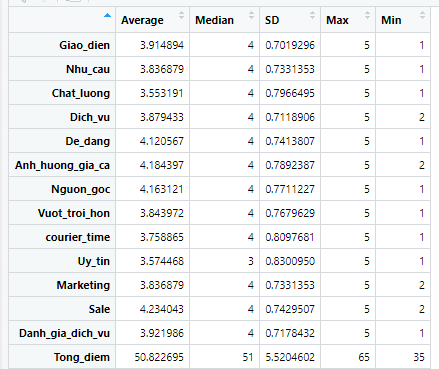
\includegraphics[scale=0.8]{rieng_3.png}
            \label{fig:my_label}
        \end{figure}
        \begin{center}
            \textbf{Hình 2: }\textit{Các thông số của các biến bình thường}
        \end{center}
\item Nhận xét: 
\begin{itemize}
    \item Dựa trên bảng kết quả, toàn bộ các thống số đều đạt khoảng giá trị điểm từ 1-5.
    \item Điểm trung bình cao nhất thuộc về biến Sale (đại diện cho các đợt khuyến mãi giảm giá)
    \item Điểm trung bình thấp nhất thuộc về biến Chat\_lương (đại diện cho chất lượng sản phẩm)
    \item Giá trị trung vị của các biến đều đạt tại 4 điểm (Mức điểm Hài lòng) ngoại trừ biến Uy\_tin (đại diện cho độ Uy tín của Shopee)
    \item Độ lệch chuẩn của các thông số không quá lớn.
    \item Như vậy, từ bảng kết quả trên, Shopee cần phải đẩy mạnh các mặt có điểm số thấp như Chất lượng sản phẩm và Uy tín của trang mạng để đáp ứng được nhiều yêu cầu của người dùng hơn.
\end{itemize}
\end{itemize}

\item Với các biến phân loại thì dùng table để thống kê số lượng
\begin{lstlisting}[language=R, caption=Làm rõ dữ liệu (tiếp theo)]
statistical_table2 <- apply(data[][1:6], 2, table)
View(statistical_table2)
\end{lstlisting}
        \begin{figure}[H]
            \centering
            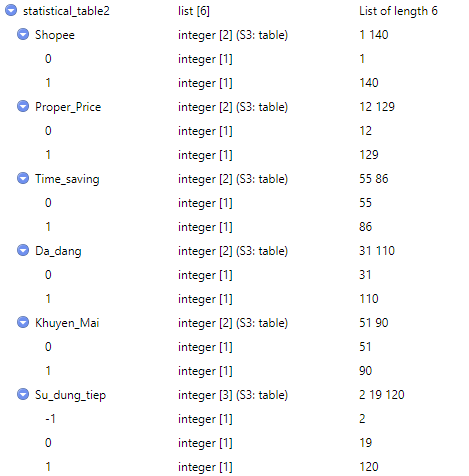
\includegraphics[scale=0.8]{rieng_4.png}
            \label{fig:my_label}
        \end{figure}
        \begin{center}
            \textbf{Hình 3: }\textit{Thống kê tần số các biến phân loại}
        \end{center}
\newpage 
\textbf{Vẽ đồ thị}
\item Thống kê phần trăm điểm tổng kết
\begin{lstlisting}[language=R, caption=Làm rõ dữ liệu (tiếp theo)]
h = hist(data$Su_dung_tiep)
h$density = h$counts/sum(h$counts)*100
plot(h,freq=FALSE, main = "Plot percent of su_dung_tiep", ylab = "%", xlab = "Quyet_dinh", border="brown", col="orange")
\end{lstlisting}
        \begin{figure}[H]
            \centering
            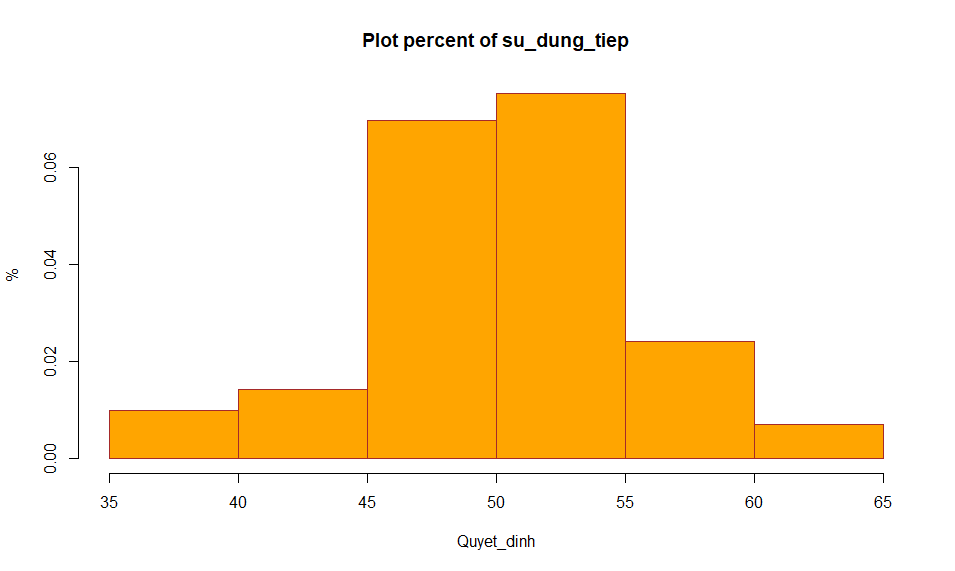
\includegraphics[scale=0.35]{rieng_plot.png}
            \label{fig:my_label}
        \end{figure}
        \begin{center}
            \textbf{Hình 4: }\textit{Đồ thị plot của biến Tong\_diem}
        \end{center}
=> Phân phối chuẩn\\
\textbf{Ta xét đến mối liên hệ giữa Tổng điểm đánh giá mà Shopee nhận được với các nội dung sau:}
\begin{itemize}
    \item Quyết định sử dụng tiếp
    \item Giá thành hợp lí
    \item Tiện lợi và tiết kiệm
    \item Tính đa dạng
    \item Khuyến mãi
    \item Điểm đánh giá Chất lượng
\end{itemize}
\item Boxplot Tổng điểm lần lượt theo các giá trị của biến "Sử dụng tiếp":
\begin{lstlisting}[language=R, caption=Làm rõ dữ liệu (tiếp theo)]
boxplot(data$Tong_diem[data$Su_dung_tiep == 1], data$Tong_diem[data$Su_dung_tiep == 0],
        data$Tong_diem[data$Su_dung_tiep == -1], main = "Boxplot Distribution of Tong_diem for Su_dung_tiep",
        at = c(1,2,3),
        names = c("Có", "Sẽ xem xét", "Không"), xlab = "Trang_thai", ylab = "Tong_diem", border="brown", col="orange")
        \end{lstlisting}
        \begin{figure}[H]
            \centering
            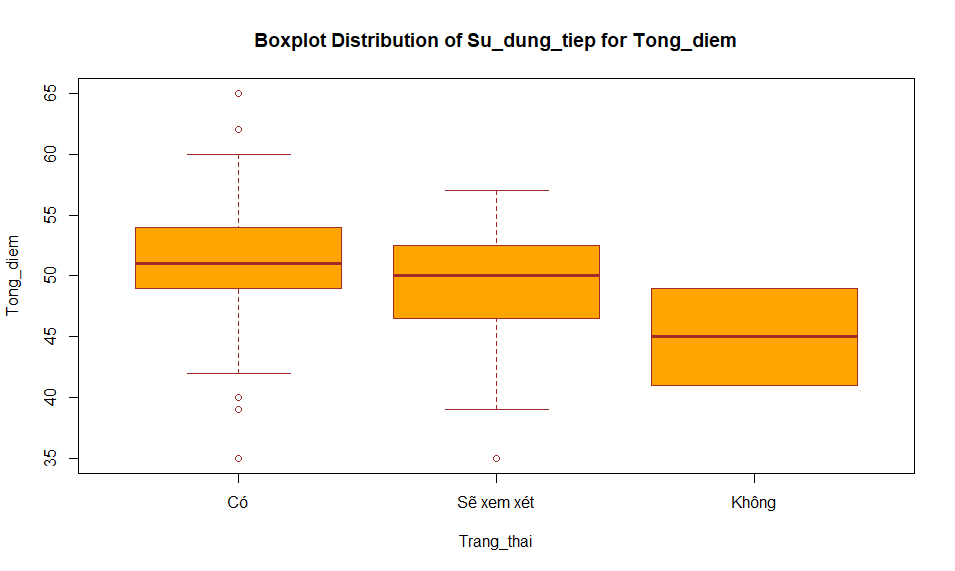
\includegraphics[scale=0.35]{a.png}
            \label{fig:my_label}
        \end{figure}
        \begin{center}
            \textbf{Hình 6: }\textit{Đồ thị boxplot của Su\_dung\_tiep tới giá trị Tong\_diem}
        \end{center}
        Và tương tự với 4 biến còn lại sẽ thu được 4 đồ thị:
        \hspace{2cm}
        \begin{figure}
\subfloat[Giá thành\label{fig:test1}]
  {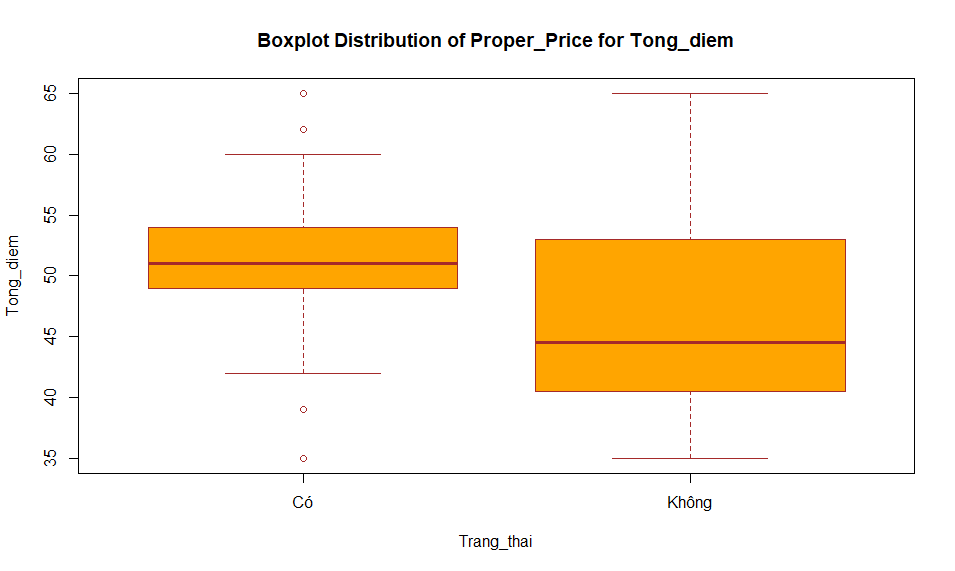
\includegraphics[width=.4\linewidth]{b.png}}\hfill
\subfloat[Tiện lợi\label{fig:test2}]
  {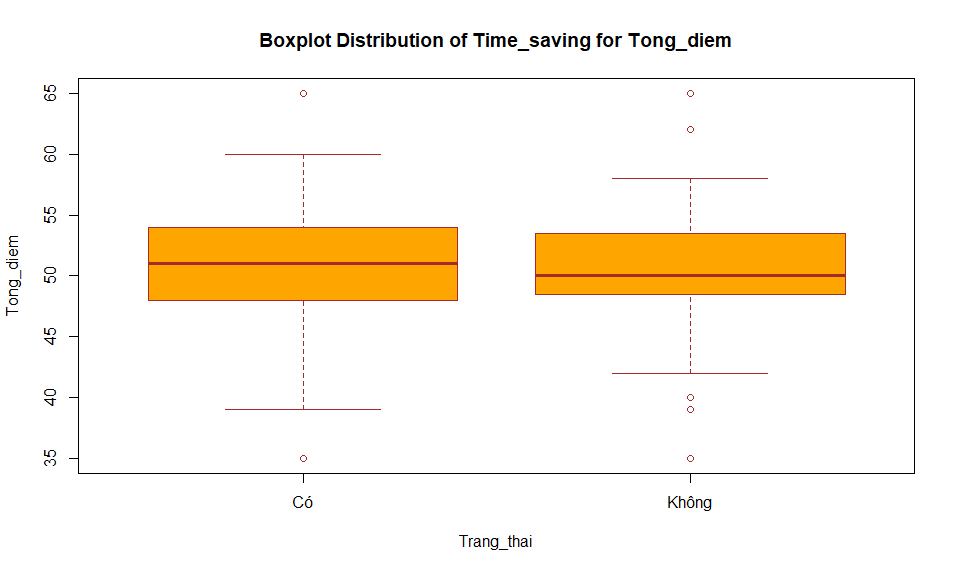
\includegraphics[width=.4\linewidth]{c.png}}\hfill
\subfloat[Đa dạng\label{fig:test3}]
  {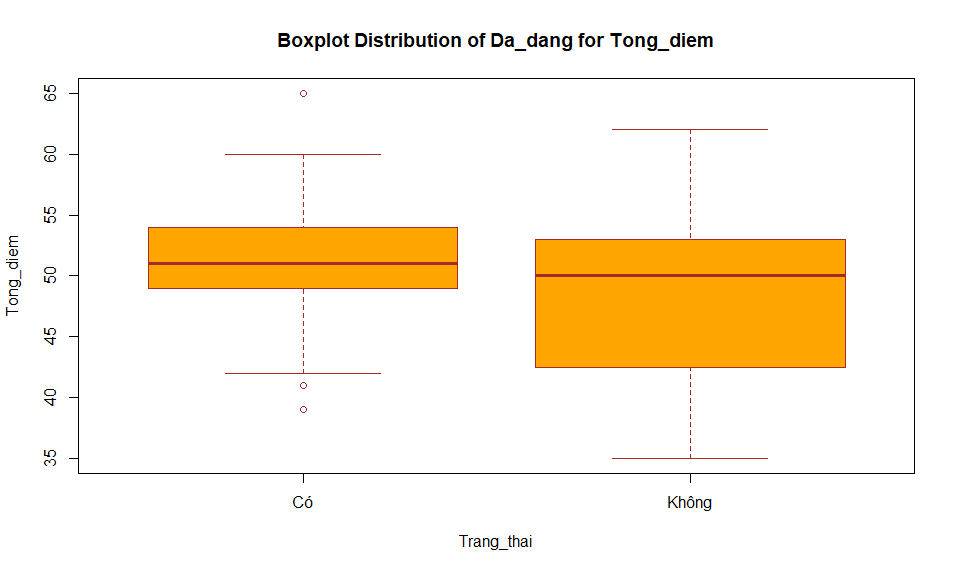
\includegraphics[width=.4\linewidth]{d.png}}\hfill
  \subfloat[Khuyến mãi\label{fig:test2}]
  {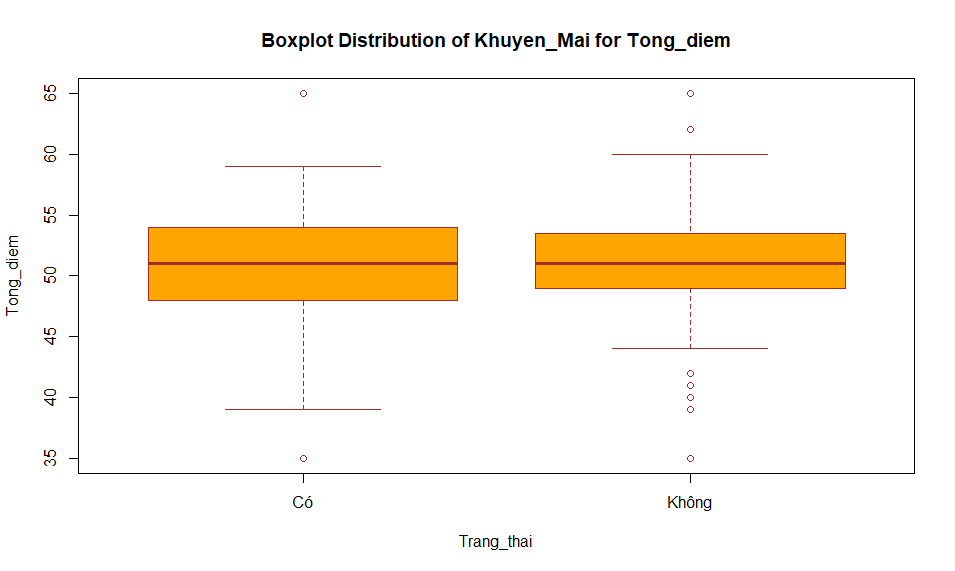
\includegraphics[width=.4\linewidth]{e.png}}\hfill
\caption{Mối liên hệ đến biến Tổng điểm}
\end{figure}

        
\text{Riêng với biến Chất lượng, ta sẽ tiến hành vẽ đồ thị thông qua hàm pairs}
    \begin{lstlisting}[language=R, caption=Làm rõ dữ liệu]
pairs(~data$Tong_diem +data$Chat_luong)
\end{lstlisting}
\begin{figure}[H]
            \centering
            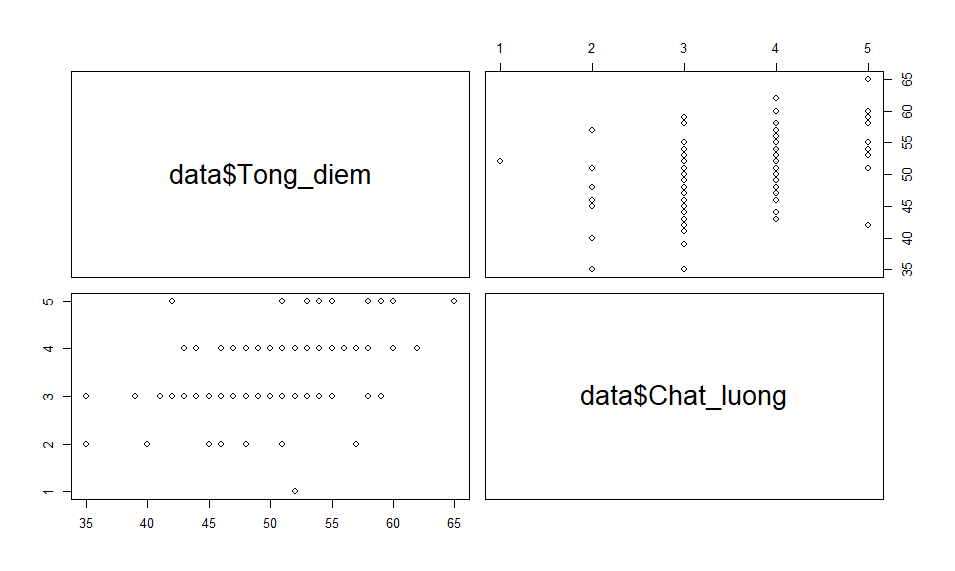
\includegraphics[scale=0.5]{6.png}
            \label{fig:my_label}
        \end{figure}



Do các giá trị của Tong\_diem phân bố ngẫu nhiên và không tạo thành hầm đường liên tục, ta có thể tiến hành mô hình hồi quy tuyến tính bội đối với giá trị định lượng là tổng điểm đối với chất lượng.\\
\end{enumerate}
    \end{itemize}
\subsection{Mô hình dữ liệu}
\begin{itemize}
Ta đưa ra giả thiết rằng: Tổng số điểm đánh giá mà Shopee nhận được là không phụ thuộc vào các đại lượng trên với độ tin cậy là 15\%\\
Xét mô hình hồi quy tuyến tính M0 như ta đã nêu..\\
    \begin{lstlisting}[language=R, caption=Mô hình dữ liệu]
# Mo hinh du lieu
new_DF = cbind( data[][2:6],data[9], data[][20])
hoiqui1=lm(Tong_diem ~. , data=new_DF )
summary(hoiqui1)
  
hoiqui2=lm(Tong_diem ~ Da_dang + Proper_Price + Chat_luong + Khuyen_Mai, data=new_DF )
summary(hoiqui2)
    \end{lstlisting}
     \begin{figure}[H]
            \centering
            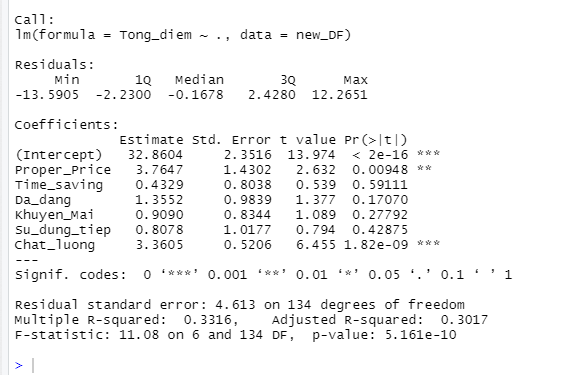
\includegraphics[scale=1]{M0.png}
            \label{fig:my_label}
        \end{figure}
    Nhận xét:\\
    \begin{itemize}
        \item Dựa trên đánh giá của hồi quy tuyến tính, Su\_dung\_tiep, Chat\_luong và Proper\_Price là các biến quan trọng.\\
        \item Khi xét thêm về t value, ta có thể nhận thêm biến Da\_dang vào nhóm này.\\
       \item Biến đại diện cho "Sử dụng tiếp" và "Tiết kiệm thời gian" có độ tin cậy thấp nên ta xem xét loại bỏ khỏi mô hình 1.\\
       \item Đồng thời ta có căn cứ để bác bỏ giả thuyết đã nêu.\\
    \end{itemize} 
    \begin{figure}[H]
            \centering
            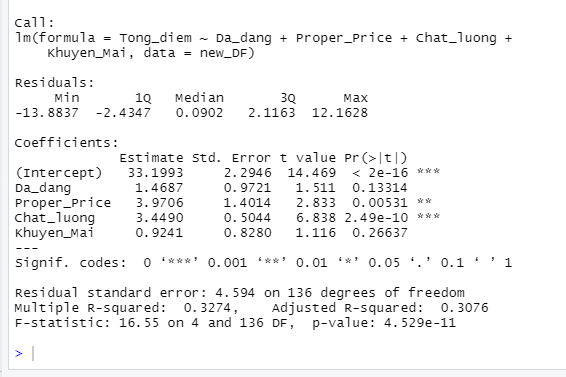
\includegraphics[scale=1]{M1.png}
            \label{fig:my_label}
        \end{figure}
        Nhận xét: 
        \begin{itemize}
            \item Xem xét đến mức độ tin cậy, các giá trị t value biến đổi nhẹ nhưng đều đạt trên ngưỡng giá trị t value của 15\%
            \item Chất lượng có ảnh hưởng rất lớn tới giá thành sản phẩm, là biến quan trọng nhất đối với mô hình trên.
            \item Như vậy, sau khi loại bỏ các biến không tin cậy mô hình 2  là mô hình hợp lí hơn.\\
        \end{itemize}
 \item Sử dụng mô hình đã lựa chọn ở trên, ta thử dự đoán giá trị tổng điểm cho Shopee khi Chất lượng bằng trung vị, các giấ trị khác đều đạt được.
    \begin{lstlisting}[language=R, caption=Mô hình dữ liệu (tiếp theo)]
predict(hoiqui2,
        data.frame( Da_dang = 1,
                    Proper_Price = 1,
                    Khuyen_Mai = 1,
                    Time_saving= 1, Su_dung_tiep = 1,
                    Chat_luong = mean(new_DF$Chat_luong)))
    \end{lstlisting}
    
    
    \begin{figure}[H]
            \centering
            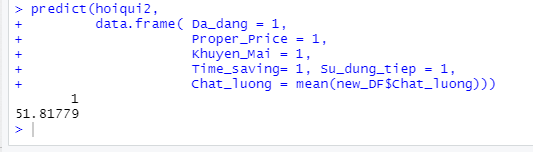
\includegraphics[scale=1]{predict.png}
            \label{fig:my_label}
        \end{figure}
    Nhận xét: \\
    \begin{itemize}
        \item Khi Shopee đạt được tất cả các khía cạnh như đa dạng, giá cả, khuyến mãi và thời gian, nếu chất lượng đạt được tại mức điểm trung bình thì tổng điểm đánh giá của Shopee là 51.82. 
    \end{itemize}
\item Thông qua bài khảo sát này, Shopee cần tập trung vào mặt chất lượng để có thể nâng điểm đánh giá của trang lên cao hơn nhằm đáp ứng nhu cầu người tiêu dùng.\\
\item Ngược lại, đối với các giá trị không chưa thoả mãn độ tin cậy, Shopee nên tiến hành cải tiến để mang lại hiệu quả cao hơn trong quá trình vận hành.\\
    
    
    \end{itemize}
\item Tổng kết:\\
\begin{itemize}
\subsection{Tổng kết:}
\item Thực hành sử dụng phần mềm RStudio
\item Thực hành phân tích dữ liệu, đánh giá các tác động 
\item Thực hành phân tích mô hình hồi quy tuyến tính và phân tích phương sai anova.
\item Thực hành nhận xét đánh giá các thông số từ mô hình được xuất ra. 
\end{itemize}
    \end{itemize}

\end{document}


